\section{Provable Security Analysis of Privacy}
\label{sec:privacy}


In this section, we will give the privacy proof and show that UPPRESSO is secure against both IdP-based login tracing and RP-based identity linkage attacks.

\noindent\textbf{IdP-based login tracing.}
As shown in figure~\ref{fig:process}, the only information that is related to the RP's identity and is accessible to the IdP is $PID_{RP}$, which is converted from $ID_{RP}$ using a random $N_U$. Since $N_U$ is randomly chosen from $\mathbb{Z}_n$ by the user and the IdP ha no control of the process, the IdP should treat $PID_{RP}$ as being randomly chosen from $\mathbb{G}$. So, the IdP cannot recognize the RP nor derive its real identity. Therefore, IdP-based identity linkage becomes impossible in UPPRESSO.

Next, we will prove that UPPRESSO prevents RP-based identity linkage based on the Decisional Diffie-Hellman (DDH) assumption \cite{GoldwasserK16}. Here, we briefly introduce the DDH assumption:
%\noindent\textbf{The DDH Assumption.}
Let $q$ be a large prime and $\mathbb{G}$ denotes a cyclic group of order $n$ of an elliptic curve $E(\mathbb{F}_q)$.
Assume that $n$ is also a large prime. Let $P$ be a generator point of $\mathbb{G}$. The DDH assumption for $\mathbb{G}$ states that for any probabilistic polynomial time (PPT) algorithm $D$, the two probability distributions \{$aP$, $bP$, $abP$\} and \{$aP$, $bP$, $cP$\}, where $a$, $b$, and $c$ are randomly and independently chosen from $\mathbb{Z}_n$, are computationally indistinguishable in the sense that there is a negligible $\sigma(n)$ with the security parameter $n$ such that:
%where $q$ and $n$ are large primitive number, and $P$ is the point of $\mathbb{G}$.
%For any probabilistic polynomial time (PPT) algorithm $D$, the distributions, \{$P$, $aP$, $bP$, $abP$\}$_{a,b \in \mathbb{Z}_n}$ and \{$P$, $aP$, $bP$, $cP$\}$_{a,b,c \in \mathbb{Z}_n}$, are computationally indistinguishable. There is a negligible $\sigma(k)$, where $k$ is the security parameter.
\vspace{-\topsep}
\begin{multline*}
Pr[D(P, aP, bP, abP)=1]-Pr[D(P, aP, bP, cP)=1]=\sigma(n)
\end{multline*}
\vspace{-\topsep}

\vspace{-2mm}
\noindent\textbf{RP-based identity linkage.}
Collusive RPs can act arbitrarily to correlate $PID_U$s at different RPs and guess if they belong to the same user. Therefore, we consider the collusive RPs are playing a guessing Game. In this Game, the IdP and the users act as the challenger, while the collusive RPs act as the adversary (denoted as $A$ in Figure~\ref{fig:game}). RP-based identity linkage is impossible in UPPRESSO {\em if and only if the adversary has no advantage over the challenger in the guessing game.}


\vspace{1mm}
\begin{strip}
\centering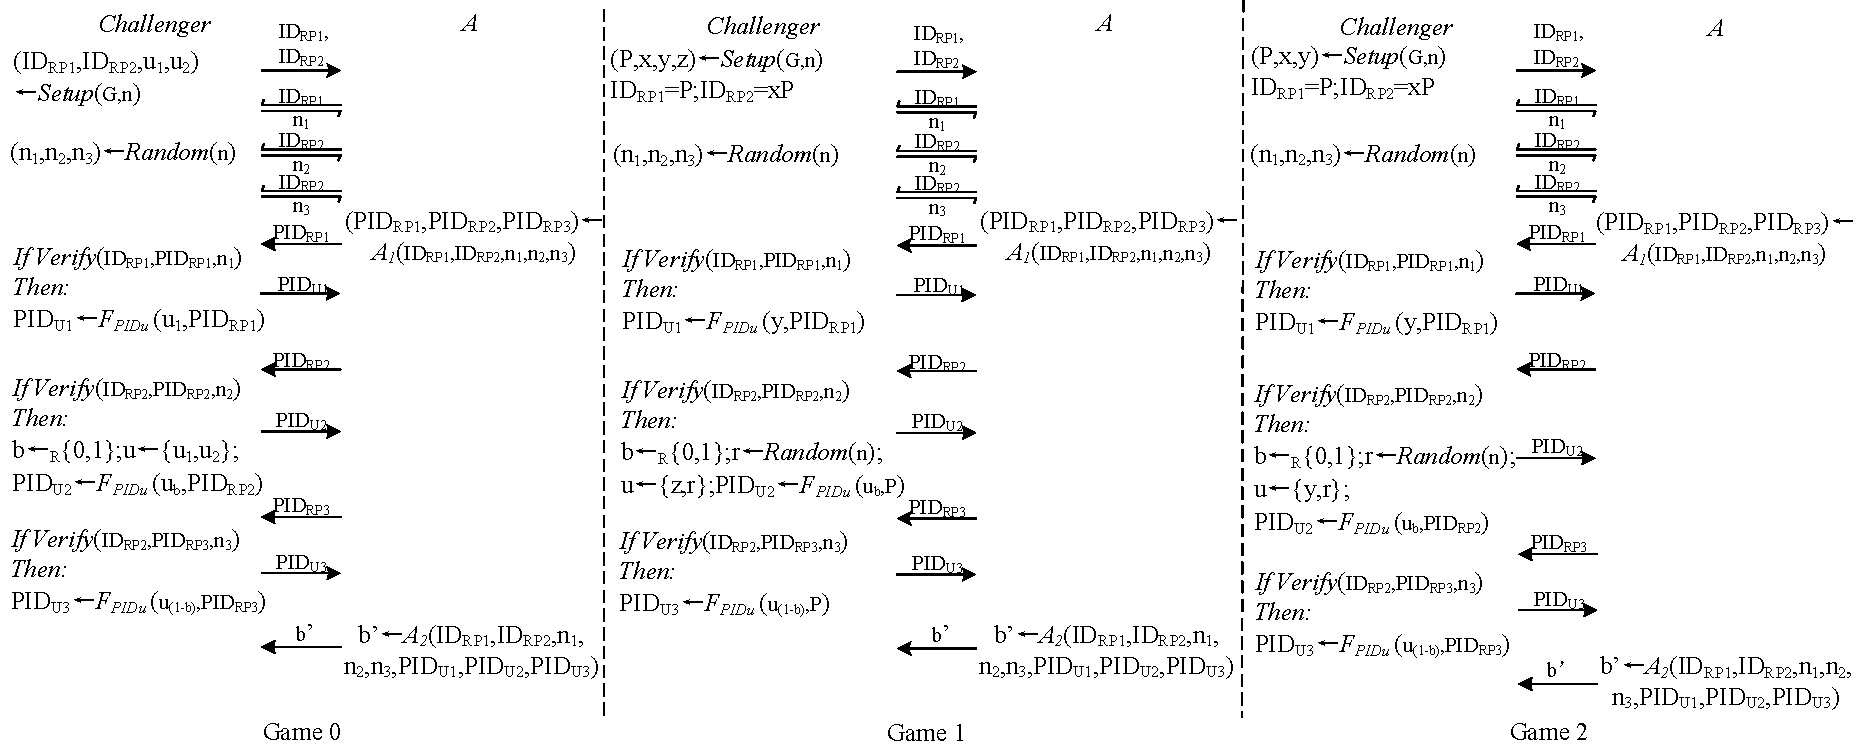
\includegraphics[width=\textwidth, height=0.35\textheight]{fig/game.pdf}
\captionof{figure}{Interactions between the challenger and the adversary in three Games.}
\label{fig:game}
\vspace{-5mm}
\end{strip}

Next, we model the guessing Game to depict the interactions between the challenger and the adversary. First, we describe the challenger's actions in the Game as follows.
\begin{itemize}
\vspace{-\topsep}
\item[-] {\em Initialization:} In initialization, the challenger generates $ID_{RP}$s and $ID_U$s for multiple RPs and users using the initialization algorithm $Setup(G,n)$, where $G$ and $n$ are defined in table~\ref{tbl:notations}.
\vspace{-\topsep}
\item[-] {\em Random number generation:} When the challenger receives the $ID_{RP}$s from the adversary, it generates a random $N_U \in \mathbb{Z}_n$ for each $ID_{RP}$ using the algorithm $Random(n)$. %$N_U$ will be used to generate the corresponding $PID_{RP}$.
\vspace{-\topsep}
\item[-] {\em $PID_U$ generation:} When the challenger receives an $PID_{RP}$, it first verifies if the $PID_{RP}$ is generated for $ID_{RP}$ with the corresponding $N_U$, using the algorithm $Verify(ID_{RP},PID_{RP},N_U)$. Then, it generates the $PID_U$ with the algorithm $F_{PID_U}(ID_U,PID_{RP})$ and sends it to the adversary.
%\vspace{-\topsep}
\end{itemize}

To prove the privacy of UPPRESSO against RP-based identity linkage, we define three Games, as shown in figure~\ref{fig:game}. First, based on the above description, we model the $ID_U$-guessing game following the UPPRESSO design as $\mathtt{Game 0}$ : (1) First, the adversary receives two $ID_{RP}$s (i.e., $ID_{RP1}$ and $ID_{RP2}$) and three $N_U$s (i.e., $n_1$, $n_2$, and $n_3$). It then generates three $PID_{RP}$s accordingly. From the challenger's view, three $PID_{RP}$s are related to three $N_U$s, respectively. (2) Then, the challenger generates $PID_U$s for different $PID_{RP}$s, using two $ID_U$s (i.e., $u_1$ and $u_2$). %generated in the initialization phase.
In particular, the challenger generates $PID_{U1}$ from $ID_{U1}$ directly, and selects a random number $b \in \{0, 1\}$ to generate $PID_{U2}=ID_{Ub} \cdot PID_{RP2}$, and $PID_{U3}=ID_{U(1-b)} \cdot PID_{RP3}$. (3) Finally, the adversary sends its guess $b'$ to the challenger. If $b'=b$, the adversary wins the game.

We define the event [$b'=b$] in $\mathtt{Game 0}$ as $\Gamma$. If the adversary has no advantage in guessing $b$ correctly, which indicates the $PID_U$s are generated from the same $ID_U$, the probability $Pr[\Gamma]$ should be 1/2. Therefore, we conclude that in $\mathtt{Game 0}$, UPPRESSO is secure against RP-based identity linkage if and only if $Pr[\Gamma]=1/2$.


Next, we build the ideal model of the guessing game, denoted as $\mathtt{Game 1}$. In this model, the probability that the adversary correctly guessing $b$ is 1/2. This time, the challenger randomly selects $z$ and $r$ and uses them to generate $PID_{U2}$ and $PID_{U3}$, respectively. Since the adversary does not know $z$ and $r$, he does not know $b$ neither. Similarly, we define the event [$b'=b$] in $\mathtt{Game 1}$ as $\Gamma_1$, and $Pr[\Gamma_1]$ should be 1/2.

According to the DDH assumption, we need to prove that $|Pr[\Gamma_1]-Pr[\Gamma]|=\sigma(n)$, where $\sigma(n)$ is negligible. So, we build another model of Game, denoted as $\mathtt{Game 2}$, by setting the values of the parameters defined in $\mathtt{Game 0}$ to be: $ID_{RP2}=xID_{RP1}$, $u_1=y$ and $u_2=r$, where $r$ is a random number. Again, we define the event [$b'=b$] in  $\mathtt{Game 2}$ as $\Gamma_2$, and $Pr[\Gamma_2]=Pr[\Gamma]$ should be true.

After defining the three games, we prove that $|Pr[\Gamma_1]-Pr[\Gamma_2]|=\sigma(n)$ as follows. In each game, the adversary uses the algorithm $A_2$ to derive $b'$ from the collected data, i.e., $\{ID_{RP1},ID_{RP2},n_1,n_2,n_3,PID_{U1},PID_{U2},PID_{U3}\}$. Now, let us replace the parameters in $\mathtt{Game 1}$ and $\mathtt{Game 2}$ with the exact values:
\vspace{-\topsep}
\begin{equation*}
\begin{aligned}
    b'_{game1} \gets A_2(P,xP,n_1,n_2,n_3,yn_1P,zP,rP) \\
    b'_{game2}\gets A_2(P,xP,n_1,n_2,n_3,yn_1P,xyn_2P,rn_3P) \\
    or \; b'_{game2}\gets A_2(P,xP,n_1,n_2,n_3,yn_1P,rn_2P,xyn_3P)
\end{aligned}
\end{equation*}
\vspace{-\topsep}

Since $n_1$, $n_2$, $n_3$ are randomly chosen by the challenger, which are not related to $ID_U$, the adversary can easily remove them and obtain $b'_{game1}\gets A_2(P,xP,yP,zP,rP)$ in $\mathtt{Game 1}$ and $b'_{game2}\gets A_2(P,xP,yP,xyP,xrP)$ in $\mathtt{Game 2}$.

As $r$ is randomly chosen and unknown to the adversary, $rP$ and $xrP$ are also random points. We can re-write $b'_{game1}$ and $b'_{game2}$ as $b'_{game1}\gets A_2(P,xP,yP,zP,r_1P)$ and $b'_{game2}\gets A_2(P,xP,yP,xyP,r_2P)$, which means there is no non-negligible difference between the success probability in $\mathtt{Game 1}$ and $\mathtt{Game 2}$, according to the DDH assumption. Otherwise, we should be able to build a PPT distinguishing algorithm that breaks DDH assumption about the adversary.

Such distinguishing algorithm $D$ is shown in figure~\ref{fig:dalgorithm}.
The inputs of the algorithm is $\{P,X,Y,Z\}$. To the adversary, it is $\mathtt{Game 1}$ if the input is in the form $\{P,xP,yP,zP\}_{x,y,z \in \mathbb{Z}_n}$, and it is $\mathtt{Game 1}$ if the input is $\{P,xP,yP,xyP\}_{x,y \in \mathbb{Z}_n}$. As a result,
\vspace{-\topsep}
\begin{multline*}
   \ \ \ \ \ \ \ \ \ \ \ \ \ \ \ \ \  Pr[D(P,xP,yP,zP)=1]=Pr[{\Gamma_1}]\\
   Pr[D(P,xP,yP,xyP)=1]=Pr[{\Gamma_2}]\ \ \ \ \ \ \ \ \ \ \ \ \ \ \ \ \ \
\end{multline*}

\vspace{-\topsep}
Therefore, $|Pr[\Gamma_1]-Pr[\Gamma_2]|=\sigma(n)$, where $\sigma(n)$ is negligible, and $n$ is the security parameter. It means the adversary has no advantage in guessing $b$ in $\mathtt{Game 0}$. Therefore, he cannot distinguish if two $PID_U$s at two different RPs belong to the same user or not. This proves that UPPRESSO is resistant to RP-based identity linkage attacks.

\begin{comment}
\begin{figure}[t]
  \centering
  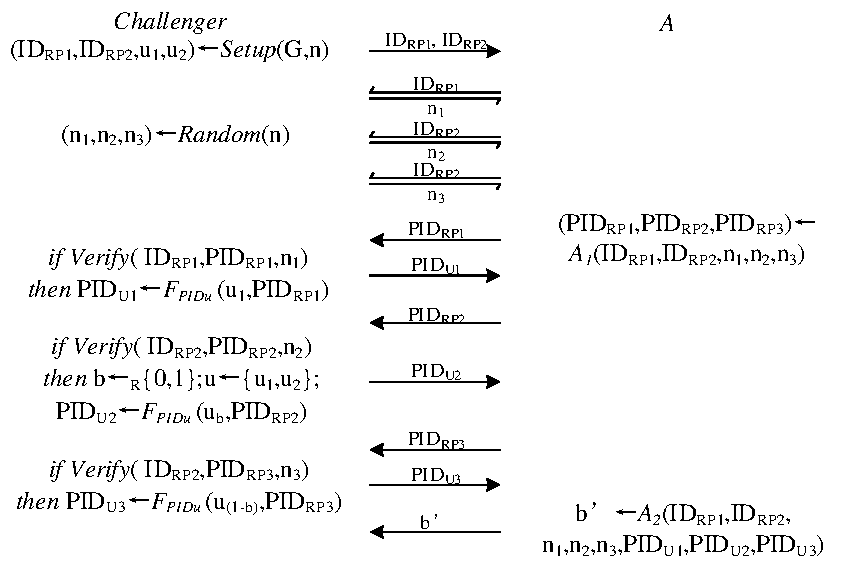
\includegraphics[width=1\linewidth]{fig/game0.pdf}
  \vspace{-5mm}
  \caption{Game 0.}
  \label{fig:game0}
  \vspace{-5mm}
\end{figure}


\begin{figure}[t]
  \centering
  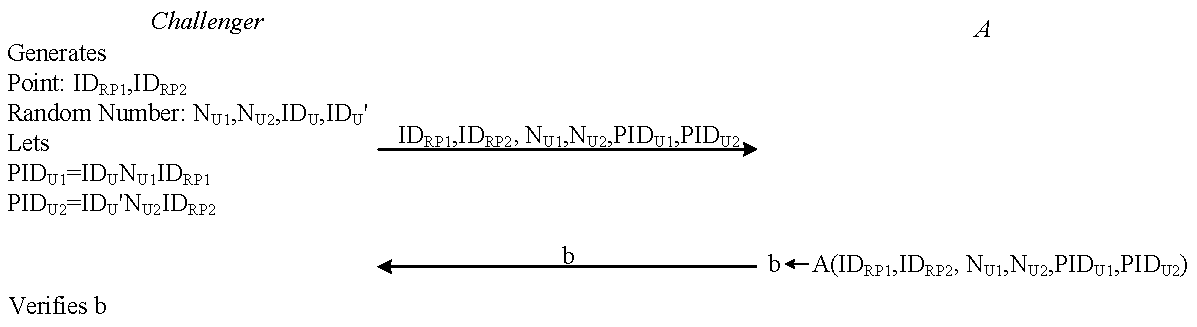
\includegraphics[width=1\linewidth]{fig/game1.pdf}
  \vspace{-5mm}
  \caption{Game 1.}
  \label{fig:game1}
    \vspace{-5mm}
\end{figure}

\begin{figure}[t]
  \centering
  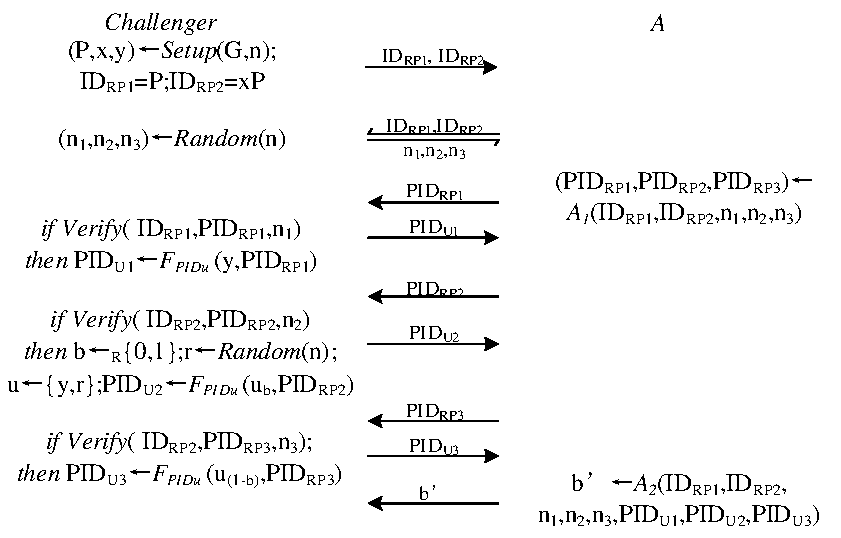
\includegraphics[width=1\linewidth]{fig/game2.pdf}
  \vspace{-5mm}
  \caption{Game 2.}
  \label{fig:game2}
  \vspace{-5mm}
\end{figure}

\end{comment}

\begin{figure}[t]
  \centering
  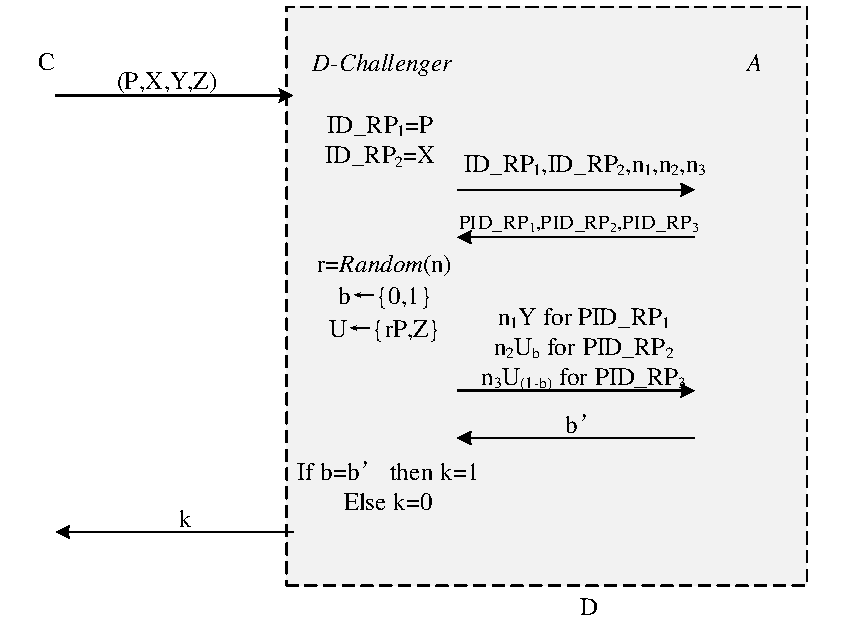
\includegraphics[width=1\linewidth]{fig/dalgorithm.pdf}
  \vspace{-5mm}
  \caption{Distinguishing algorithm.}
  \label{fig:dalgorithm}
  \vspace{-5mm}
\end{figure}
